\documentclass{memoriaPFC}
\fontfamily{cmss}\selectfont



%
% DATOS DEL DOCUMENTO
%

\title{Colmena: diseño e implementación de un widget web para micro donaciones, con página web de soporte, almacenamiento de datos y su posterior visualización}

%\autores{Nombre1 Apellidos1}{Nombre2 Apellidos2} Hasta 5 autores
\autores{Rubén Sánchez Corcuera}{}{}{}{}

%El director del proyecto
\director{Pablo García Bringas}
%\directora{Ursula K. Le Guin}

% iaei ii ioi itel (ii es un pdf que contiene los logos para el grado de informatica, el unico actualizado)
\titulacion{ii}

% mayo || septiembre (en minúsculas!!)
\date{mayo de 2017}

\resumen{%
 El proyecto consta de varios módulos. La base de todo es un servidor implementado en node.js. En él se aloja la página web, los widgets de las diferentes empresas que han decidido implantarlo en sus páginas web y una restful API que administra el enrutamiento de la web y permite varias funciones sobre la base de datos.\\
 
 La página web sirve de apoyo al widget, es donde se muestra la información general del widget, los diferentes proyectos a los que apoyar, un wizard con el que poder crear tu propio widget y la plataforma para poder conseguir el certificado de donación.\\
 
 La base de datos noSQL aloja los datos de las diferentes donaciones para posteriormente poder crear el certificado de donación y eventualmente generar estadísticas sobre las cantidades, fechas y lugares en los que más donaciones se están obteniendo.\\
 
 Por último, el widget. Está pensado para que las empresas que tengan portales de compra online lo incrusten durante algunas de sus fases compra del cliente con el fin de que este haga una pequeña donación a la causa que las empresas han “apadrinado”. El widget es personalizable por las empresas que lo quieran implantar en su web, así conseguir una mayor integración con ellas. Entre sus opciones de personalización destaca la posibilidad de elegir entre una cantidad fija o variable de donación.
  
 
}
\descriptores{solidaridad, widget, RESTful, NodeJS, MongoDB}


%
% COMIENZO DEL DOCUMENTO
%
\begin{document}

% Portada, resumen, indices
\frontmatter
\hacerportada
\hacerresumen
\tableofcontents
\listoffigures % Opcional
\listoftables % Opcional
%\lstlistoflistings % Opcional

% Contenidos
\mainmatter
\chapter{Introducción}

\section{Presentación del documento}

El presente documento recoge la definición de objetivos del proyecto que realizará el alumno Rubén Sánchez para la ONG ALBOAN. En el proyecto consta de todo el sistema necesario para crear un sistema de micro donaciones mediante un widget 5 en cualquier tienda online. El sistema consta de: una página web, una base de datos, el widget y un servidor que da soporte a todo. Además, el sistema cuenta con una funcionalidad añadida por la que se puede crear gráficas de visualización.\\

El proyecto se desarrolla para la ONG Alboan la cual al ver el cambio que se da en la sociedad en materia de solidaridad y que las grandes donaciones han sufrido una gran caída decide que la manera de recoger las donaciones tiene que cambiar. Alboan, al explorar las oportunidades y ver que la única opción disponible cobra a las ONGs un porcentaje de las donaciones decide crear un sistema de micro donaciones gratuito que cualquier empresa pueda añadir a su tienda online y así fomentar las donaciones a pequeña escala, consiguiendo así que el 100\% del dinero vaya al destino final.\\

Los principales capítulos del documento son los siguientes:

\begin{itemize}
	\item \textbf{Introducción} \smallbreak
	 En este apartado se incluye una visión global del documento y del proyecto que se va a llevar a cabo.
	\item \textbf{Demandante del proyecto} \smallbreak
	 En este apartado se hará una descripción sobre la empresa demandante.
	 \item \textbf{Situación de partida} \smallbreak
	 En este apartado se trata la motivación por la que se va a desarrollar el proyecto, con esto también se analizan las posibles soluciones dadas para el problema y por últimos los objetivos que se quieren conseguir.
	\item \textbf{Definición del proyecto}\smallbreak
	Este es el apartado más importante del documento, en él se describe el producto final que se va a generar y la metodología utilizada para desarrollarlo.
	\item \textbf{Condiciones de ejecución}\smallbreak
	En este apartado se describen los materiales utilizados para desarrollar el proyecto, el hardware necesario para su puesta en marcha y el equipo que lo desarrollará.
	\item \textbf{Presupuestos y tiempos} \smallbreak
	En este apartado se describen los gastos que puede tener el proyecto en materia de tareas y equipo utilizado para desarrollarlo.
\end{itemize}


\chapter{Objetivos del proyecto}

\smallbreak %borrar
En este capítulo hablaremos sobre el beneficiario del proyecto, en este caso es la ONG ALBOAN.

\section{Alboan}

La actividad de Alboan comenzó en 1994, asumiendo las iniciativas de voluntariado
internacional que ya estaban en marcha, pero fue en 1996 cuando se configuró
jurídicamente bajo la figura de Fundación. Es la ONG promovida por la Compañía de Jesús en la Provincia de Loyola (País Vasco y Navarra). El nombre, en euskera, Alboan, quiere reflejar el arraigo a la cultura de la tierra vasca y el espíritu de la entidad: estar al lado de las personas más excluidas, junto a organizaciones y centros educativos.\\

Su logo(Figura \ref{logo}) visibiliza  el rol de bisagra y puente que quería jugar la institución para poner en relación dos mundos que en realidad son uno solo. Su misión: ser plataforma de encuentro de personas y organizaciones de aquí y allá que quisieran comprometerse en la construcción de un mundo mejor.\\

Hoy Alboan cuenta con 7000 personas entre contratados, voluntarios y entidades que le permiten apoyar y acompañar a más de 200 proyectos llevados a cabo por 105 organizaciones
aliadas que impactan directamente en las vidas de más de 600.000 personas en todo
el mundo.

\figura{0.5}{imgs/alboan.jpg}{Logo de Alboan}{logo}{}

\subsection{Misión y Visión}

\subsubsection{Misión}

Trabaja por la construcción de una ciudadanía global que denuncie las injusticias que provocan desigualdad en el mundo, construya una cultura que promueva el bien común y transforme las estructuras generadoras de pobreza a nivel local y global. Para lograrlo, se une en red con personas y grupos de todo el mundo.\\

La colaboración de Alboan se centra en 4 temáticas principales en las que enmarca todos sus proyectos y labores de ayuda: Educación de calidad, Desarrollo económico-productivo sostenible y equitativo, Acción humanitaria en crisis recurrentes y Democracia a favor de las personas excluidas.\\

Todas las actividades que realiza la ONG incluyen 3 ejes transversales que otorgan a los proyectos el carisma que Alboan quiere dar:
\begin{itemize}
	\item La espiritualidad como dimensión en el horizonte de desarrollo humano.
	\item El reconocimiento de las desigualdades entre mujeres y hombres y el compromiso con la equidad de género.
	\item La participación ciudadana para la incidencia social y política.
\end{itemize}

\subsubsection{Visión}

Lograr una Alboan que contenga las siguientes características:
\begin{itemize}
	\item \textbf{Enraizada} en el nuevo proyecto unificado de la Compañía de Jesús a través de sus plataformas locales y territorial.
	\item \textbf{Querida} por las organizaciones y la base social con las que se alía.
	\item \textbf{Reconocida} por su valor añadido en el acompañamiento a entidades, la
	formación y la construcción de ciudadanía global.
	\item \textbf{Sostenible} gracias a un equipo comprometido y una financiación estable y
	diversificada.
	\item \textbf{Ilusionante}, por sus propuestas y su comunicación esperanzadora.
	\item \textbf{Puente} entre nuestro estilo de vida y las situaciones de frontera de
	deshumanización
\end{itemize}


\subsection{Dedicación}

Alboan tiene unos ámbitos de dedicación marcados en los que

\begin{itemize}
	\item La \textbf{Cooperación al Desarrollo} en África, Asia, Centroamérica y Sudamérica, principalmente con proyectos educativos, de promoción económica y de formación de grupos excluidos para la defensa de sus derechos.

	\item La \textbf{Educación para la solidaridad} en Euskadi y en Navarra, mediante la participación en campañas, la elaboración de materiales educativos, la promoción del comercio justo, impartiendo formaciones y talleres y asesorando a grupos y centros educativos.

	\item La \textbf{Acción Política} participando en redes y elaborando estudios e investigaciones para incidir y mejorar las políticas que afectan al desarrollo tanto locales como internacionales.


\end{itemize}


\chapter{Situación de partida}

\small %Quitar
En este capítulo se habla sobre la necesidad de la cual surge crear este proyecto, la motivación por la cual se decide desarrollar el producto final y los objetivos que se pretender conseguir con el mismo.

\section{Necesidades}





Años atrás Alboan comienza a detectar una bajada en la forma tradicional de hacer donaciones. Es entonces cuando se plantea buscar nuevos métodos para realizar estas donaciones y que el dinero siga fluyendo. En el ejercicio de 2015 la financiación privada fue ligeramente menor que el año anterior y se rompió la tendencia en alza. A parte de tener menos financiación Alboan se da cuenta de que algunos de sus proyectos no son conocidos y que la ayuda para que estos continúen es crucial, por lo que la preocupación hacia estos proyectos crece.\\

Es entonces cuando le surgen a Alboan varias necesidades, la de volver a conseguir financiación privada ya que no pueden sustentarse únicamente de los legados solidarios y las cuotas que pagan sus socios y por otra parte la de hacer llegar a más personas sus proyectos para que de esta manera aumente su sensibilidad con el tema. Para lograr cubrir estas necesidades Alboan intenta pensar en una solución en la que los proyectos de la ONG se den a conocer y que la gente que este interesada en ellos pueda hacer una pequeña aportación, en este momento surge la idea de las pequeñas donaciones.\\


\newpage

\section{Objetivos}

El principal objetivo de este proyecto es crear un widget solidario que se pueda implantar en cualquier tienda online y crear la página web en la que se va a apoyar y se dará a conocer este widget. La página web también será el portal en el que la gente que ha realizado alguna donación pueda recoger su certificado de donación con el fin de presentarlo en la declaración de la renta.\\
Otro objetivo sería el de crear el servidor con la base de datos para alojar los datos de las donaciones realizadas mediante el widget. Este servidor seria accesible para las personas de Alboan que quisieran consultar los datos de las donaciones o ver las gráficas relacionadas con esto.  \\

\section{Requerimientos}

En este apartado listaremos los diferentes requerimientos del proyecto.

\begin{itemize}
	\item Formar a las personas que realizarán el mantenimiento del sistema mediante tutoriales.
	\item Utilizar las últimas tecnologías en diseño web.
	\item Crear una web responsiva para que todos los usuarios puedan acceder a ella y que evite la brecha digital.
	\item Garantizar los tiempos de respuesta del widget para que las empresas que lo usen no vean perjudicados sus comercios online.
	\item Visualización de datos comprensible e intuitiva.
\end{itemize}

\section{Estado del arte}
En este apartado se hace un análisis de las diferentes opciones que hay para cubrir las necesidades citadas anteriormente.
\subsection{Crowdfunding}
“Cooperación colectiva, llevada a cabo por personas que realizan una red para conseguir dinero u otros recursos, se suele utilizar Internet para financiar esfuerzos e iniciativas de otras personas u organizaciones”\cite{crowd}\\

En el crowdfundig hay diferentes tipos de ayudas y de sistemas creados para financiar los proyectos que la gente sube a las plataformas: basado en donaciones (migranodearena, teaming...), basados en recompensas(Goteo, Verkami...) y para préstamos(ECrowd!) entre otros.

\subsubsection{Basado en donaciones}
El usuario realiza una donación para ayudar a un proyecto que le gusta y no recibe ningún beneficio económico en retorno (solo la satisfacción de hacer algo bueno y de apoyar un proyecto que le emociona). Son proyectos solidarios con un impacto social grande.
\begin{itemize}
	\item \textbf{Migranodearena.org:}\smallbreak
	La página web migranodearena es un proyecto creado por la Fundación Privada real dreams. Es una plataforma de crowdfunding solidario, pionera en España, abierta para todas las Entidades No Lucrativas, legalmente constituidas y con sede en España. \\
	En migranodearena se puede liderar un reto y recaudar fondos en grupo a favor de una ONG. Una persona o grupo de personas, lanza un reto en migranodeareana para apoyar una causa solidaria. Comparte el reto con todos sus familiares, amigos, conocidos, clientes, empleados, proveedores y entre todos suman granitos de arena.
	\item \textbf{Teaming:}\smallbreak
	Teaming es una herramienta online para recaudar fondos para causas sociales a través de micro donaciones de \EUR{1} al mes. La filosofía de Teaming se basa en la idea de que con \EUR{1}, nosotros solos no podemos hacer mucho pero si nos unimos, podemos conseguir grandes cosas.\\
	El sistema de funcionamiento de Teaming es muy sencillo, puedes publicar un grupo en el que la gente se apunte y done \EUR{1} al mes o puedes apuntarte a un grupo que otra persona haya publicado para donar tu ese euro. Entre las ideas clave mas destacadas de la plataforma están la de solo donar \EUR{1} al mes, ni más ni menos y la de solo aceptar causas sociales.
\end{itemize}

\subsubsection{Basado en recompensas}
Se trata de aportar dinero a un proyecto y se recibe a cambio una recompensa. Los proyectos pueden consistir en crear y diseñar un nuevo producto o financiar un proyecto cultural (película, festival, musical). Es el modelo de crowdfunding más utilizado y conocido. En cada proyecto se puede elegir entre un rango de recompensas en función de la cantidad de dinero que se aporte.

\begin{itemize}
	\item \textbf{Goteo:} \smallbreak
	A simple vista, Goteo es una plataforma de crowdfunding cívico y colaboración en torno a iniciativas ciudadanas, proyectos sociales, culturales, tecnológicos y educativos. Con réplicas y alianzas en varios países, gracias a su código abierto, además de reconocida y premiada internacionalmente desde 2011. Constituye una herramienta de generación de recursos, gota a gota, para una comunidad de comunidades compuesta por más de 65.000 personas, con un porcentaje de éxito de financiación superior al 70\%.\\
	Pero en realidad Goteo es mucho más que eso. Tras la plataforma existe una fundación sin ánimo de lucro y un equipo multidisciplinar desde el que desarrollan herramientas y servicios de co-creación y financiación colectiva. Con una misión común vinculada siempre a principios de transparencia, progreso y mejora de la sociedad.
\end{itemize}

\subsubsection{Para prestamos}
El usuario realiza una inversión en un proyecto o en una empresa de la plataforma y recibe un retorno económico en forma de intereses. La empresa contrata un préstamo con la plataforma de crowdlending, que lo gestiona, y el usuario recupera el dinero invertido junto a los intereses a lo largo del tiempo según las condiciones pactadas en el préstamo.

\begin{itemize}
	\item \textbf{ECrowd!:} \smallbreak
	ECrowdInvest es una plataforma de crowdlending (crowdfunding en forma de préstamo) para proyectos con impacto social y medio ambiental positivo (lo que venimos a llamar impacto positivo). Es una clara versión del clásico "win-win", donde todos ganan, ya que los buenos proyectos consiguen financiarse, los inversores reciben unos intereses mucho más altos de los que se obtienen con los bancos y siempre se genera un impacto positivo sobre el medio ambiente, por ejemplo, en la financiación colectiva de proyectos que impliquen la reducción de emisiones de dióxido de carbono hacia la atmósfera.
\end{itemize}


\subsection{Micro donaciones}

Las micro donaciones, como su nombre indica, son donaciones muy pequeñas realizadas con el fin de aportar una pequeña cantidad de dinero al proyecto que nos interesa. En este ámbito nos encontramos con Worldcoo una herramienta online con bastante recorrido y reconocimiento.

\begin{itemize}
	\item \textbf{Worldcoo:} \smallbreak
	Worldcoo es una empresa nacida en 2012 que pretende crear un nuevo canal de financiación mediante un widget incrustado en tiendas online. Esto permite que las miles de personas que acceden y compran en las tiendas online puedan donar una pequeña cantidad al proyecto que esa página tiene apadrinado.\\
	Cuentan con un extenso equipo de personas y de embajadores en varios paises del mundo, lo que les da acceso a muchos comercios online. Las empresas contactan con Worldcoo y acuerdan entre los dos la instalación del widget en su tienda online. Este widget esta relacionado con uno de los proyectos de las ONGs a las que Worldcoo ayuda.
\end{itemize}

Esto es exactamente lo que Alboan quiere, pero tiene algunas carencias. La empresa Worldcoo se queda un 8\% de las donaciones realizadas a cada proyecto por lo que esto empieza a disgustar a Alboan, esta empresa tampoco permite ver las personas que están donando a los proyectos por lo que no permite mantener el contacto con esas personas para hacerles conscientes de que su ayuda tiene un resultado. \\

Después de hacer un análisis de todas las opciones y ver los resultados Alboan decide crear su propia plataforma de micro donaciones mediante widgets en tiendas online.


\chapter{Definición del proyecto}

\small %quitar
En este apartado se procede a definir el proyecto, la metodología utilizada para desarrollarlo y el alcance del mismo. Durante todo el desarrollo del proyecto y las decisiones tomadas en el mismo se ha tenido en mente lo escrito en este apartado.

\section{Descripción del producto}

En este apartado se presenta una descripción completa del producto final, el cual consta de 4 partes, que juntas, forman el sistema completo Colmena.\\

El sistema Colmena consta de las 4 partes que se muestran en la Figura 4.1. El servidor central que une las otras 3 partes es el núcleo del proyecto. A este servidor se conectan los otros 3 componentes de la infraestructura completa a las que el servidor otorga funcionalidad. En la página web se permite al usuario informarse sobre los proyectos y sobre el proyecto Colmena en general. También ofrece la expedición de certificados y la creación de nuevos widgets. En la base de datos se almacenan los datos respectivos a las donaciones y a los donantes, en este caso el servidor extrae e introduce datos en ella para poder gestionar los certificados de donación. Por último, el widget, este es el producto final que la mayoría de los usuarios verán. Este se coloca en los comercios online para que las personas puedan hacer una pequeña aportación a los proyectos que la tienda haya apadrinado.

\begin{figure}[h]
	\centering
	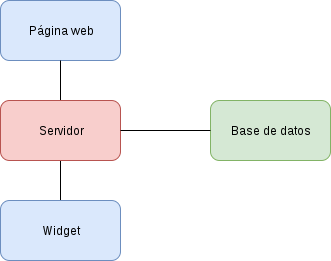
\includegraphics[width=0.5\textwidth]{imgs/descripcion.png}
	\caption{Infraestructura de Colmena}
	\label{infraestructura}
\end{figure}

\subsection{Widget}
El widget es la parte principal del proyecto. Es el objeto que las empresas colocaran en sus tiendas online y que permitirá a los clientes hacer una donación. Consiste en un pequeño rectángulo(\ref{widget}) en el que se le ofrece al a persona que está leyéndolo que aporte una pequeña cantidad de dinero, siempre entre 1 y 5 euros, a un proyecto en concreto. \\

El widget es 100\% personalizable. En la web existe un asistente que permite a las empresas personalizar el widget de modo que este encaje bien en sus comercios online. Este asistente permite cambiar las siguientes características del widget:

\begin{itemize}
	\item \textbf{Proyecto:} Permite elegir a que proyecto destinar el dinero entre los proyectos de Alboan.
	\item \textbf{Opciones de donación:} Permite decidir si la donación será estática, de \EUR{1}, o si esta podrá ser variable, entre 1 y 5 euros.
	\item \textbf{Fondo:} Permite elegir entre una foto, única para cada proyecto, o un fondo de color estático mediante un selector de color.
	\item \textbf{Color de la fuente:} Permite elegir el color de la fuente
\end{itemize}

El widget está compuesto de lenguaje HTML5 y CSS3, no tiene ningún plugin externo, lo que permite incrustarlo en cualquier página web sin que esta se vea afectada o haya que hacer alguna modificación en ella. Se ha desarrollado para que sea responsivo.\\

Por último, la inclusión del widget en la tienda esta simplificada al máximo de manera que la tienda no se vea afectada o tenga que realizar labores de reestructuración del código de su página web. Este proceso se hace mediante un script de código en JavaScript que permite añadir, en el espacio reservado para el mismo, el widget.

\begin{figure}[h]
	\centering
	
\includegraphics[width=1\textwidth]{imgs/widget.png}
	\caption {Widget Colmena}
	\label{widget}
\end{figure}



\subsection{Pagina web}

La página web de la Colmena cubre las labores de publicidad y de soporte del widget. Esta incluye funcionalidades como recoger el certificado de donación después de haber realizado una, crear nuevos widgets para las empresas que quieran añadirlos a su página web o contacto con el soporte de Alboan.\\

La página esta desarrollada en \textit{HTML5}, \textit{CSS3}(mediante el pre procesador \textit{sass}) y \textit{JavaScript}. A parte de estas tecnologías se ha utilizado el framework web \textit{Bootstrap} y una gran cantidad de plugins que permiten una mejor navegabilidad en la página web, entre ellos destaca \textit{JQuery}. Se han seleccionado estas tecnologías tras una investigación sobre las tecnologías más recomendadas para el tipo de proyecto. Dado que no teníamos ningún requerimiento sobre estas, hemos apostado por las tecnologías que más nos apetecía utilizar, innovando en algunas de las situaciones y siendo más conservadores en otras.\\

La página web permite al usuario consultar cierta información y realizar varias opciones. Estas opciones se explican a continuación:

\begin{itemize}
	\item \textbf{Conocer el proyecto Colmena:} Es el comienzo de la página web, tras la introducción, compuesta por una foto, está localizada este apartado. Aquí se explica el funcionamiento y la filosofía del proyecto Colmena.
	\item \textbf{Conocer proyectos de Alboan:} En este apartado se exponen los diferentes proyectos que dispone la ONG Alboan. Los proyectos están expuestos con el nombre de este y el país en el que actúa. Si hacemos clic en cualquiera de los proyectos una ventana se despliega y ofrece más información sobre este.
	\item \textbf{Crear un widget:} En este apartado de la página web se ofrece la posibilidad de crear un widget personalizado. Al hacer clic en el botón que ofrece esta posibilidad se despliega una ventana con un asistente. En este asistente se ofrecen varias opciones para personalizar el widget final. Este asistente no es el definitivo que las empresas usaran para realizar el widget que quieren que sea colocado en su comercio online.
	\item \textbf{Recibir un certificado:} En este apartado los usuarios pueden utilizar el código de donación que reciben al donar en cualquier tienda que tenga implantada la Colmena. Después de introducir los datos en un formulario, se le enviará el certificado de donación al mail que ha especificado.
	\item \textbf{Contactar con el soporte de Colmena:} Este es el último apartado de la página web. En él se puede enviar un mail al soporte de Colmena. Es el método de interlocución entre las empresas que quieran implantar el widget en sus comercios y el soporte de Colmena.
\end{itemize}
\newpage
\subsection{Base de datos}

La base de datos de la Colmena está desarrollada en la base de datos NoSQL por excelencia, MongoDB. Se ha utilizado este tipo de base de datos por la versatilidad que proporciona a la hora de acceder a los datos y al conectarse a ella. Es una base de datos muy ágil por lo que permite consultar en un tiempo muy reducido las donaciones. Por último, se ha utilizado esta base de datos por la experimentación con la misma, al no ser una base de datos SQL el equipo tuvimos las ganas de probarla y ver su potencial.\\

La base de datos se encarga de almacenar todos los datos relativos a las donaciones mediante los siguientes campos:

\begin{itemize}
	\item \textbf{Importe:} El importe de la donación.
	\item \textbf{Usada:} Un booleano que marca si la donación ha sido canjeada por el certificado o no.
	\item \textbf{Fecha:} La fecha dividida por día, mes y año.
	\subitem Día
	\subitem Mes
	\subitem Año
	\item \textbf{idDonacion:} Un id asignado a cada donación.\\
\end{itemize}

Una vez almacenada la donación esta está disponible para canjearla por un certificado de donación en la página web. Una vez el certificado de donación es expedido, los datos de la persona donante se guardan en la base de datos con el fin de hacerle llegar información sobre los proyectos, si así lo desea, o hacer diferentes estadísticas con las que la organización pueda mejorar o cambiar sus métodos. Estos son los datos que se añaden al archivo de la donación:

\begin{itemize}
	\item DNI/CIF: Número de identificación fiscal de la persona física o jurídica.
	\item Nombre y Apellidos: El nombre y los apellidos de la persona física o nombre de la empresa.
	\item Razón social: Denominación por la cual se conoce colectivamente a la empresa y en caso de ser una persona, introducirá la palabra "Individuo"
	\item Correo electrónico
	\item Dirección
	\item Código Postal
	\item Población
	\item Provincia
\end{itemize}


\subsection{Servidor}


El servidor del proyecto es el núcleo del mismo. En el convergen todas las funcionalidades de la solución. Este está desarrollado en Node.js. Tras una investigación de las posibles tecnologías y tras ver que no había requerimientos en este aspecto decidimos utilizar esta herramienta ya que es innovadora y emergente.\\

La funcionalidad que el servidor ofrece a los demás componentes del proyecto se basa en recabar la información necesaria de la base de datos y ofrecérsela a la página web para que esta la utilice en sus funciones. También recaba la información del widget y se lo envía a la base de datos para que esta la almacene. Por último el servidor también se utiliza como sistema de almacenamiento de los widgets para tenerlos centralizados y poder repararlos rápidamente en caso de error.\\

El servidor se desarrolla de esta manera, como pieza central, por el hecho de unificar todas las funcionalidades que el sistema pueda necesitar en el mismo nodo. Gracias a la flexibilidad de Node.js y a los plugins que se ofrecen en \textit{NPM}, el gestor de paquetes para \textit{JavaScript}. Con estos plugins se ha conseguido unificar todas las funcionalidades que sin ellos habría que haber desarrollado mediante otros métodos, por ejemplo, el envío de mails o el sistema de creación del certificado de donación.

\subsection{Visualización}

La visualización de los datos es la parte final del proyecto. Este módulo permite visualizar mediante una serie de gráficos interactivos los datos de las donaciones. Los gráficos, como ya he dicho anteriormente son interactivos para que los usuarios puedan 'jugar' con ellos e ir relacionando los datos. Estos gráficos están divididos en dos:

\begin{itemize}
	\item \textbf{Gráfico de queso:} En este gráfico interactivo los usuarios pueden ir clusterizando la información en diferentes divisiones. La primera división por ejemplo seria la dividir las donaciones por el proyecto al que han donado y posteriormente se podría ir profundizando en más opciones.
	\item \textbf{Gráfico con mapa:} En este gráfico se puede ver un mapa de calor en el que se pueden ver las zonas desde las que más se ha donado.
\end{itemize}

Posteriormente estos gráficos se pueden analizar para sacar conclusiones de ellos y poder ofrecer esta información de vuelta a los donantes y socios de la ONG. Con esta información los donantes pueden ver lo que la entidad está recibiendo y como es la sociedad que les rodea gracias al mapa de calor. Por último, Alboan podrá analizar esta información y tomar algunas decisiones basándose en ella además de añadirla a los informes que publica.


\newpage

\subsubsection{Investigación sobre las tecnologías a utilizar}
En esta tarea se investigarán las principales tecnologías a utilizar en el proyecto principal. Se buscarán las mejores tecnologías para desarrollar un proyecto web integral. Las principales funciones de las tecnologías serán las siguientes, crear un servidor web, crear una página web, crear un widget responsivo que se comunique con el servidor y crear una base de datos que aloje los datos.

\subsubsection{Redactar el documento sobre las tecnologías a utilizar}
En esta tarea se redactará lo decidido en la tarea anterior. Se explicarán las diferentes tecnologías que se utilizarán y porque se han elegido estas.

\subsubsection{Instalar las herramientas de desarrollo}
En esta tarea se instalarán las herramientas pertinentes para el desarrollo del proyecto y su correspondiente gestión.

\subsubsection{Configurar la herramienta de control de versiones}
En esta tarea se instalará la herramienta seleccionada anteriormente para el control de versiones en online. Ya que en el desarrollo estarán implicadas más de una persona, se utilizará una herramienta de este tipo para controlar más el desarrollo.

\subsubsection{Diseñar la arquitectura del proyecto}
El objetivo de esta tarea será el de crear una arquitectura completa del proyecto que tenga en cuenta todos los elementos de este. Se crearán los diferentes proyectos en las herramientas de programación, con los métodos más generales. También habrá que crear las conexiones entre las diferentes tecnologías.

\subsubsection{Crear el primer diseño de la página web}
En esta tarea se crearán varios mockups para la interfaz de la página web, que luego serán entregados al cliente para que este las revise y decida cual desea.

\subsubsection{Crear el primer diseño del widget}
En esta tarea se crearán varios mockups para la interfaz del widget, que luego serán entregados al cliente para que este las revise y decida cual desea.

\subsubsection{Desarrollar la lógica del servidor}
En esta tarea se desarrollarán todos los métodos y servicios que el servidor tenga que implementar para dar servicio a todos los componentes del proyecto.

\subsubsection{Pruebas servidor}
En esta tarea se deberá probar el servidor ante todo tipo de situaciones para evitar fallos futuros.

\subsubsection{Configurar la base de datos}
En esta tarea se deberá configurar la base de datos para que sea capaz de alojar los datos que el servidor, el widget y la página web.

\subsubsection{Pruebas base de datos}
En esta tarea se deberá probar la base de datos ante todo tipo de situaciones para evitar fallos futuros.

\subsubsection{Desarrollar la lógica de la página web}
En esta tarea se desarrollará el sistema de enrutado y de funcionalidad de la página web.

\subsubsection{Desarrollar la lógica del widget}
En esta tarea se desarrollará la funcionalidad y la conexión con el servidor del widget.

\subsubsection{Consolidar el diseño de la página web}
En esta tarea se establecerá el diseño definitivo de la página web.

\subsubsection{Pruebas de la página web}
En esta tarea se deberá probar la página web ante todo tipo de situaciones para evitar fallos futuros.

\subsubsection{Consolidar el diseño del widget}
En esta tarea se establecerá el diseño definitivo de la página web.

\subsubsection{Pruebas del widget}
En esta tarea se deberá probar el widget ante todo tipo de situaciones para evitar fallos futuros.

\subsubsection{Crear manual de usuario para los técnicos de mantenimiento}
En esta tarea se deberá crear un manual que indique detalladamente como son todos los procesos que hay que realizar para mantener el sistema y crear nuevos widget para las empresas.

\subsubsection{Investigar los frameworks de visualización de datos}
En esta tarea se deberán investigar los frameworks que se utilizarán a posteriori para visualizar los datos extraídos de las donaciones. Los gráficos deberán ser interactivos.

\subsubsection{Configurar el framework de visualización de datos}
En esta tarea se configurará el framework elegido en la tarea anterior.

\subsubsection{Pruebas sobre el framework de visualización de datos}
En esta tarea se deberá probar el framework de visualización de datos ante todo tipo de situaciones para evitar fallos futuros.

\subsubsection{Analizar los datos}
En esta tarea se analizarán los datos extraídos de la base de datos y se cargarán en diagramas para su posterior visualización.

\subsubsection{Extraer las estadísticas de los datos}
En esta tarea se deberán extraer conclusiones de los datos y análisis realizados en la anterior tarea. Se deberá realizar un documento que recoja las conclusiones extraídas del proceso de análisis de los datos.



\chapter{Condiciones de ejecución}

El desarrollo tendrá lugar en Deusto Tech. Aquí es donde tendrá su lugar de trabajo el equipo. El proyecto se desarrollará en el transcurso del año 2016-2017.DeustoTech y Alboan ofrecerán todos los medios necesarios para el buen desarrollo del proyecto.

\section{Instalaciones}
En este apartado se listará el software y hardware utilizado para desarrollar el proyecto.

\subsection{Hardware}
Este es el hardware que se utilizará para desarrollar el proyecto:
\begin{itemize}
	\item Lenovo ThinkPad X220
	\item Monitor Acer AL1714 (Segundo monitor)
\end{itemize}

\subsection{Software}
Este es el software que se utilizará para desarrollar el proyecto. Este sera explicado mas adelante:
\begin{itemize}
	\item Atom
	\item MongoDB
	\item Git
	\item Brackets
\end{itemize}

\subsubsection{Atom}
Atom es un editor de código fuente abierto para macOS, Linux, y Windows con soporte para plug-ins escrito en Node.js, Incrustando Git Control, desarrollado por GitHub. Atom es una aplicación de escritorio construida utilizando tecnologías web. La mayor parte de los paquetes tienen licencias de software libre y es construido y mantenido por su comunidad. Atom está basado en Electrón (Anteriormente conocido como Atom Shell), Un framework que permite aplicaciones de escritorio multiplataforma usando Chromium y Node.js. Está escrito en CoffeeScript y Less. También puede ser utilizado como un entorno de desarrollo integrado (IDE). Atom libero su beta en la versión 1.0, encima junio 25, 2015. Sus desarrolladores lo llaman un "Editor de textos hackable para el siglo XXI".


\subsubsection{MongoDB}
MongoDB es un sistema de base de datos NoSQL orientado a documentos, desarrollado bajo el concepto de código abierto. MongoDB forma parte de la nueva familia de sistemas de base de datos NoSQL. En lugar de guardar los datos en tablas como se hace en las bases de datos relacionales, MongoDB guarda estructuras de datos en documentos similares a JSON con un esquema dinámico (MongoDB utiliza una especificación llamada BSON), haciendo que la integración de los datos en ciertas aplicaciones sea más fácil y rápida.

\subsubsection{Git}
Git es un software de control de versiones diseñado por Linus Torvalds, pensando en la eficiencia y la confiabilidad del mantenimiento de versiones de aplicaciones cuando éstas tienen un gran número de archivos de código fuente. Al principio, Git se pensó como un motor de bajo nivel sobre el cual otros pudieran escribir la interfaz de usuario o front end como Cogito o StGIT. Sin embargo, Git se ha convertido desde entonces en un sistema de control de versiones con funcionalidad plena. Hay algunos proyectos de mucha relevancia que ya usan Git, en particular, el grupo de programación del núcleo Linux.


\subsubsection{Brackets}
Brackets es un editor de codigo fuente abierto escrito en HTML, CSS y JavaScript enfocado en el diseño web. Fue creado por Adobe Systems, bajo licencia del MIT y actualmente mantenido por GitHub. Brackets está disponible para Mac, Windows y Linux.




\section{Equipo de proyecto}
En este apartado se describirá al equipo del proyecto desde dos perspectivas diferentes. En la sección de Interacción con el cliente se describirá como deberá ser el contacto con el cliente poniendo en práctica las buenas prácticas de la metodología Scrum. En el caso de los perfiles profesionales se definirán los perfiles que deberá haber para desarrollar el proyecto y cómo será el organigrama del proyecto.

\subsection{Interacción con el cliente}
El esquema organizativo

\begin{itemize}
	\item \textbf{Product Owner:} Este rol será representado por una persona de Alboan. Sus principales funciones son las siguientes:
		\subitem Ser el representante de todas las personas interesadas en los resultados del proyecto
		\subitem Definir los objetivos del producto o proyecto.
		\subitem Colaborar con el equipo para planificar, revisar y dar detalle a los objetivos de cada iteración.
	\item \textbf{Scrum master:} No se debe confundir con el jefe de proyecto. Sus principales tareas son:
		\subitem Facilitar las reuniones de Scrum
		\subitem Proteger y aislar al equipo de interrupciones externas
		\subitem Quitar los impedimentos que el equipo tiene en su camino
	\item \textbf{Equipo de desarrollo:} Compuesto por los profesionales que desarrollarán el proyecto. Su principal función es desarrollar el proyecto y estas son otras de sus funciones:
		\subitem Equipo auto organizado.
		\subitem Equipo multidisciplinar, capacidad de desarrollar diferentes tareas.
		\subitem Equipo estable durante el proyecto y establecidos en la misma localización física.

\end{itemize}

En la figura 5.1 se puede ver cómo será la interlocución entre los miembros del equipo. El Scrum master, representado por Rubén Sánchez, será el encargado de interaccionar con el Product Owner, que estará representado por una persona de Alboan. Por último, el equipo de desarrollo incluirá a las personas que desarrollen el proyecto, las cuales podremos ver más adelante.

\figura{0.6}{imgs/equiposcrum.png}{Gráfico de la interacción en el proyecto}{equiposcrum}{}

\subsection{Perfiles profesionales}

En este apartado se describirá al equipo de proyecto que será el encargado de desarrollar el producto y los diferentes perfiles necesarios para ello.

\begin{itemize}
	\item \textbf{Jefe de proyecto:} Es el encargado de controlar que el proyecto se desarrolle correctamente y de garantizar los tiempos de desarrollo y la calidad del mismo. También se encargará de los aspectos de gestión del proyecto.
	\item \textbf{Diseñador:} Es el encargado de diseñar la interfaz de la página web y del widget.
	\item \textbf{Analista de datos:} Es el encargado de analizar los datos que se extraen del proyecto y de crear informes interactivos y conclusiones de ellos.
	\item \textbf{Arquitecto web:} Es el encargado de diseñar y desarrollar la arquitectura principal del proyecto. También se encarga de configurar las herramientas que vayan a utilizar los demás para asegurar su correcto funcionamiento.
	\item \textbf{Programador:} Es el encargado de desarrollar los métodos que el arquitecto haya establecido.
\end{itemize}

En la figura 5.2 se ve la organización en el equipo de proyecto. Alboan está como cliente externo a Deusto Tech. Dentro de Deusto Tech tenemos a Pablo García, el cual será el supervisor del proyecto desde la empresa, y al equipo de la Colmena. Dentro del equipo de la Colmena contamos con dos personas, el jefe del proyecto, que hará las veces de Diseñador, Analista de datos y Arquitecto Web y, por otra parte, el programador.

\figura{0.8}{imgs/Equipo.png}{Gráfico del equipo de proyecto}{equipo}{}

\subsection{Procedimientos de seguimiento y control}

El seguimiento del proyecto se hará desde el tablón de Trello. En el tablón se registran los cambios que se generan y se generan notificaciones para las personas involucradas en la tarea que ha sufrido cambios. Finalmente se puede sacar un reporte de los cambios en las tareas.\\

En cuanto a reuniones de seguimiento del proyecto, tendremos una reunión cada viernes en la que el equipo de proyecto hablará con el supervisor de Deusto Tech. En esa reunión se podrán ver los avances y problemas que hay cada semana y se pensarán diferentes soluciones para ellos. Estas reuniones también servirían por si se necesitará algo de Deusto Tech.


\chapter{Planificación}


En este capítulo hablaremos sobre la planificación y presupuestos del proyecto.

\section{Presupuesto}
En este apartado se detalla el coste en días de cada tarea. Cada día está compuesto por 8h laborales. Cada tarea será realizada por un perfil profesional, cobrando cada uno su precio en horas.

\figuraSinMarco{1}{imgs/tareas.png}{Lista de tareas con su coste en horas}{tareas}{}

\begin{table}[]
	\centering
	\begin{tabular}{llll}
		\textbf{Perfil profesional} & \textbf{Horas} & \textbf{Precio (por horas)} & \textbf{Importe} \\
		Diseñador                   & 120            & 20                          & 2400             \\
		Arquitecto web              & 136            & 20                          & 2720             \\
		Programador                 & 240            & 20                          & 4800             \\
		Analista de datos           & 120            & 25                          & 3000             \\
		\hline Precio total                &                &                             & 12920
	\end{tabular}
	\caption{Presupuesto del proyecto desglosado}
	\label{precios}
\end{table}


\section{Planificación del proyecto}

En la figura 6.2 se puede ver el diagrama Gantt del proyecto. Este está divido en los 4 sprints de los que antes hemos hablado. Las barras negras corresponden a los sprints, cada uno de los sprints esta compuesto por unas barras que indican la duración de las tareas dentro de ellos. Las flechas indican la precedencia de las tareas

\figuraSinMarco{0.7}{imgs/gantt.png}{Diagrama Gantt}{gantt}{}

\section{Justificación financiera}

Este proyecto no genera beneficios ya que se trata de una plataforma para obtener donaciones para otros proyectos, por lo que el dinero recaudado por la plataforma está directamente destinado a los proyectos. Por otra parte, la plataforma ofrecerá numerosos beneficios a la ONG ya que hará más visibles sus proyectos y ofrecerá una manera más fácil de hacer donaciones a las personas que estén interesadas. También unificará la manera de recibir estas donaciones y las tendrá todas almacenadas en un sistema completo por lo que hacer estudios sobre estas donaciones será muy sencillo.


\chapter{Especificación de requisitos}

\section{Visión general}

En este capitulo se especifican los requisitos que el proyecto debe satisfacer y que definen el funcionamiento de todo el software que compone este proyecto. Para una mejor compresión de los mismos, se dividen en los siguientes bloques:

\begin{itemize}
	\item \textit{Especificación de requisitos del servidor Node.js:} en esta sección se recogen los requisitos que debe de satisfacer el servidor, este es el encargado de soportar todo el sistema.
	\item \textit{Especificación de requisitos de la página web:} en esta sección se recogen los requisitos que debe satisfacer la página web del proyecto.
	\item \textit{Especificación de requisitos del widget:} en esta sección se recogen los requisitos que debe satisfacer el widget del proyecto, el elemento que estará incrustado en las tiendas online.
	\item \textit{Especificación de requisitos de la base de datos:} en esta sección se recogen los requisitos que debe satisfacer la base de datos, esta albergará los datos de las donaciones y donantes.
	\item \textit{Especificación de requisitos del sistema de visualización:} en esta sección se recogen los requisitos que debe satisfacer el sistema de visualización, el encargado de crear gráficas interactivas para la visualización y estudio de los datos.
\end{itemize}

\section{Especificación de requisitos del servidor Node.js}
Los requisitos funcionales del servidor Node.js son:

\begin{itemize}
	\item \textbf{RF.0.1} El servidor debe ser capaz de albergar la página web.
	\item \textbf{RF.0.2} El servidor debe ser capaz de albergar las rutas de la página web y ofrecer el enrutamiento a cada una de estas.
	\item \textbf{RF.0.3} El servidor debe ser capaz de conectarse con la base de datos.
	\item \textbf{RF.0.4} El servidor debe ser capaz de enviar mails.
	\item \textbf{RF.0.5} El servidor debe ser capaz de alterar un PDF.
	\item \textbf{RF.0.6} El servidor debe ser capaz de crear un script y almacenarlo.
	\item \textbf{RF.0.7} El servidor debe ser capaz de ofrecer un script a páginas de terceros.
	\item \textbf{RF.0.8} El servidor debe ser capaz de ofrecer datos a una tercera aplicación.
\end{itemize}

Los requisitos no funcionales son:

\begin{itemize}
	\item \textbf{RNF.0.1} Mantenibilidad: el sistema tiene que tener un mantenimiento sencillo ya que tiene conexiones con paginas de terceros lo que obliga a que el mantenimiento sea sencillo y rápido.
	\item \textbf{RNF.0.2} Escalabilidad: el servidor tiene que ser escalable ya que la creación de nuevos widgets o la oferta de datos a terceras aplicaciones puede ser grande.
\end{itemize}



\section{Especificación de requisitos de la página web}

Los requisitos funcionales de la página web son:

\begin{itemize}
	\item \textbf{RF.1.1} La página web debe ofrecer un wizard para la creación de nuevos. widgets
	\item \textbf{RF.1.2} La página web debe ofrecer un formulario para la obtención de un certificado de donación.
	\item \textbf{RF.1.3} La página web debe ofrecer un sistema para comunicarse con el soporte del proyecto.
\end{itemize}

Los requisitos no funcionales de la página web son:

\begin{itemize}
	\item \textbf{RNF.1.1} La página web debe informar sobre el proyecto.
	\item \textbf{RNF.1.2} La página web debe informar sobre los proyectos de la ONG.
	\item \textbf{RNF.1.3} Accesibilidad: La página web tiene que ser responsiva para ser adaptable en diferentes dispositivos.
	\item \textbf{RNF.1.4} Interfaz: la página web debe tener un diseño simple para facilitar la navegación.
	\item \textbf{RNF.1.5} Escalabilidad: la página tiene que ser escalable ya que se tienen que poder añadir nuevos proyectos a ella.
\end{itemize}

\section{Especificación de requisitos del widget}

Los requisitos funcionales del widget son:

\begin{itemize}
	\item \textbf{RF.2.1} El widget debe permitir la donación fija o variable de una cantidad de dinero.
	\item \textbf{RF.2.2} El widget debe ser de fácil implantación por parte de la tienda online.
\end{itemize}

Los requisitos no funcionales del widget son:

\begin{itemize}
	\item \textbf{RNF.2.1} El widget debe informar sobre el proyecto al que va destinado.
	\item \textbf{RNF.2.2} Accesibilidad: el widget debe ser responsivo para que pueda añadirse en cualquier tienda.
	\item \textbf{RNF.2.3} Interfaz: el widget debe ser 100\% personalizable.
	\item \textbf{RNF.2.4} Disponibilidad: el widget debe estar disponible en todo momento para su uso por parte de los comercios online.
\end{itemize}

\section{Especificación de requisitos de la base de datos}

Los requisitos funcionales de la base de datos son:

\begin{itemize}
	\item \textbf{RF.3.1} La base de datos debe almacenar los datos de las donaciones.
	\item \textbf{RF.3.2} La base de datos debe almacenar los dados de los donantes.
	\item \textbf{RF.3.3} La base de datos debe proporcionar los datos que se le pidan.
\end{itemize}

Los requisitos no funcionales de la base de datos son:

\begin{itemize}
	\item \textbf{RNF.3.1} Rendimiento: la base de datos debe almacenar y proporcionar los datos en un tiempo razonable.
	\item \textbf{RNF.3.2} Seguridad: la base de datos debe ser segura para no poner en peligro los datos de los donantes.
	\item \textbf{RNF.3.3} Disponibilidad: La base de datos debe estar disponible para almacenar las donaciones e información de donantes.
\end{itemize}

\section{Especificación de requisitos del sistema de visualización}

Los requisitos funcionales del sistema de visualización son:

\begin{itemize}
	\item \textbf{RF.4.1} El sistema de visualización debe ofrecer gráficos interactivos.	
	\item \textbf{RF.4.2} El sistema de visualización debe conectarse con el servidor para adquirir los datos.
\end{itemize}

Los requisitos no funcionales del sistema de visualización son:

\begin{itemize}
		\item \textbf{RNF.4.1} Escalabilidad: el sistema de visualización de datos debe ser escalable ya que los datos pueden crecer y la manera de mostrarlos cambiar.
		\item \textbf{RNF.4.2} Interfaz: el sistema de visualización de datos debe tener una interfaz intuitiva que permita una buena navegación por los gráficos.
\end{itemize}

\chapter{Tecnologías utilizadas}

En esta sección se presentan las diferentes tecnologías que se han usado para el desarrollo del proyecto. Las principales tecnologías utilizadas son las siguientes:

\section{Node.js}
Esta es la autodefinición que se hace Node.js en su propia página web:

\begin{quote}
	Node.js\cite{wsdl13} es un entorno de ejecución para JavaScript construido con el motor de JavaScript V8 de Chrome. Node.js usa un modelo de operaciones E/S sin bloqueo y orientado a eventos, que lo hace liviano y eficiente. El ecosistema de paquetes de Node.js, npm, es el ecosistema mas grande de librerías de código abierto en el mundo.\\
\end{quote}


Node.js es una solución con un solo hilo de ejecución que permite que las peticiones a esta no bloqueen peticiones futuras ni exige grandes pools de hilos para tener conexiones concurrentes. Esto permite que los comercios onlines conecten con el servidor y le hagan una petición para recibir el widget a lo que el servidor responderá con el envió y el cierre de la conexión, evitando así el cuello de botella que se puede generar con conexiones masivas.\\

Node.js cuenta con un gestor de paquetes llamado npm del que se pueden descargar diferentes modulos para ampliar la funcionalidad de esta tecnología. Gracias a este gestor de paquetes node.js se convierte en una solución integral para la parte servidora habilitándole con todo lo necesario para cumplir las funciones del backend de una solución web.

Entre las ventajas que ofrece Node.js se encuentran las siguientes:

\begin{itemize}
	\item \textbf{Gran documentación:} tiene una gran documentación y 8 años de experiencia por lo que la mayoría de los casos y posibilidades están testadas haciendo su desarrollo mas sencillo.
	\item \textbf{Gran comunidad:} gracias al gestor de paquetes publico y a los años de experiencia Nodejs cuenta con una gran comunidad con la que poder consultar las dudas y usos de los diferentes paquetes.
	\item \textbf{npm:} su gestor de paquetes publico  permite reutilizar código y no perder tiempo implementando código que ya ha sido desarrollado y probado anteriormente.
	\item \textbf{Multiplataforma y open-source:} esta desarrollado para ser utilizado en cualquier sistema operativo y cuenta con una licencia MIT, lo cual lo hace gratuito y permite arreglar e incluso mejorar el propio código de la herramienta por los usuarios de esta.
\end{itemize}

\subsection{Funcionamiento}
En Node.js es muy sencillo crear aplicaciones nuevas que actuen en la parte servidora de una aplicación. Gracias a npm, Node.js es muy polivalente, pero a continuación se mostrará un ejemplo de un servidor HTTP:

\begin{codigo}
http.createServer(function (request, response) \{
	response.writeHead(200, {'Content-Type': 'text/plain'});
	response.end('Hello World');
\}).listen(8081);
console.log('Server running at http://127.0.0.1:8081/');
\end{codigo}

En este ejemplo se crea un servidor HTTP en el puerto 8081 de la maquina local. Una vez se entra al puerto 8081 de la maquina local, el servidor creara una respuesta en texto plano y la enviará al navegador, que mostrará por pantalla el mensaje.\\

Node.js funciona de una manera muy diferente dependiendo de los paquetes utilizados para el desarrollo de la aplicación por lo que a continuación explicare los paquetes utilizados para el desarrollo de este proyecto y como es el funcionamiento de cada uno de estos:

\subsection{Express}
Express es un framework web minimalista y flexible para el desarrollo de soluciones web en node.js. Express además aplica una fina capa con las características fundamentales de las aplicaciones web sobre la base de node.js permitiendo así mantener todas las funcionalidades que ofrece Node.js. Finalmente, Express ofrece una amplia y robusta API para hacer uso de todas las funcionalidades y características que ofrece.

\subsubsection{Funcionamiento}
Express no tiene una estructura de proyecto definida por los desarrolladores o comunidad, en cambio, tanto en la documentación como en numerosos sitios ofrecen un sistema de carpetas para tener el proyecto ordenado y las rutas definidas.

\begin{codigo}
	project/
	|--	node\_modules/
	|--	public/
			 |--	images/
			 |--	css/
			 |--	javascript/
	|--	routes/
	|--	views/
	|--	app.js
	|--	package.json
\end{codigo}

\begin{itemize}
	\item \textbf{Node\_modules:} en esta carpeta irán incluidas todas las dependencias del proyecto una vez descargadas automáticamente por npm.
	\item \textbf{Public:} en esta carpeta estarán los elementos de uso publico por parte del proyecto, imágenes, scripts de JavaScript y hojas de estilo.
	\item \textbf{Routes:} aquí se encuentran las rutas a las diferentes entidades en archivos diferentes.
	\item \textbf{Views:} en esta carpeta estarán incluidas las vistas del proyecto, es decir, las diferentes pantallas de la página web.
	\item \textbf{App.js:} es el archivo principal del proyecto.
	\item \textbf{Package.json:} es un archivo de configuración general del proyecto, en el irán las dependencias y los metadatos del proyecto.
\end{itemize}

\subsubsection{Razón de uso}
Se ha elegido este framework ante otros disponibles para Node.js por varias razones:

\begin{itemize}
	\item El primer commit de esta herramienta fue 2 meses después de la creación de Node.js y la primera versión 1 año después por lo que tiene un gran recorrido y madurez.
	\item Su sencillez para manejar las rutas y las vistas en una solución web.
	\item Gran comunidad de desarrolladores en la que apoyarse.
\end{itemize}

\subsection{Express-ejs-layouts}

\subsection{Nodemailer}
Nodemailer es un módulo para Node.js que permite enviar emails. Este módulo esta securizado de manera que los mensajes que envía los hace de manera segura. Permite adjuntar elementos a los mensajes y no depende de ningún otro paquete, lo que le convierte en un paquete muy completo.

\subsubsection{Funcionamiento}
Nodemailer es muy sencillo de usar, solo hay que definir el mensaje con los campos y archivos adjuntos que quieras añadir y también habrá que definir el transporter que sera el encargado de enviar el mensaje. En este caso no esta añadido la configuración del transporter.

\begin{codigo}
	var message = \{
		from: 'sender@server.com',
		to: 'receiver@sender.com',
		subject: 'Message title',
		text: 'Plaintext version of the message',
		html: '<p>HTML version of the message</p>'
	\};
	transporter.sendMail(data);
\end{codigo}

\subsubsection{Razón de uso}
Se ha utilizado este paquete para enviar los mails por su sencillez, el gran recorrido que tiene en esta materia, ya que fue creado en 2010 y por su completa documentación.

\subsection{Mongojs}
Mongojs es un paquete para Node.js que permite la conexión con bases de datos MongoDB. Este paquete intenta emular completamente la comunicación directa con la base de datos por lo que su API se asemeja mucho a la de MongoDB.

\subsubsection{Funcionamiento}
Mongojs es muy sencillo de usar, con la siguiente linea de código, conectaremos con una base de datos MongoDB que este en un servidor remoto y si añadimos la variable mycollection, conectaremos directamente con la colección dentro de la base de datos elegida. 

\begin{codigo}
	var db = mongojs('example.com/mydb', ['mycollection'])
\end{codigo}

A continuación se muestra un ejemplo en el que se busca en la base de datos todos los documentos en los que name=Jhon. Esta función devuelve los documentos que cumplan la condición y posteriormente se pueden tratar dentro de la función.

\begin{codigo}
	  db.mycollection.find(\{ 'Name':'Jhon'\}function (err, docs) \{
	  	// Insert code here 
	  \});
\end{codigo}

\subsubsection{Razón de uso}
Se ha utilizado este paquete para conectar con la base de datos por la facilidad con la que conecta con la base de datos y porque emula lo máximo posible la API de mongoDB haciendo su uso muy fácil si ya has utilizado mongoDB con anterioridad.

\subsection{Pdffiller}
Pdffiller es un paquete para Node.js que permite rellenar los formularios de los PDF’s con datos. Su uso se basa en recibir PDF’s con formularios sin rellenar, unos datos y combinarlos de manera que la salida sea un PDF completo. 

\subsubsection{Razón de uso}
Se ha utilizado este paquete por ser el mas utilizado por los usuarios entre las posibilidades. 

\section{MongoDB}
MongoDB es la base de datos NoSQL líder y permite a las empresas ser más ágiles y escalables. Organizaciones de todos los tamaños están usando MongoDB para crear nuevos tipos de aplicaciones, mejorar la experiencia del cliente, acelerar el tiempo de comercialización y reducir costes.\\

Es una base de datos muy ágil por lo que permite cambiar los esquemas al cambiar los requisitos y a la vez proporciona las mismas funcionalidades que se esperan de una base de datos tradicional, manteniendo la velocidad en las búsquedas y siendo consistente.\\

Gracias a ser una base de datos orientada a documentos no hay que ajustarse a un esquema estándar ni obligar a todos los registros a tener la misma información. Esto nos da mucha flexibilidad a la hora de querer introducir nuevos datos o alterar los que ya tenemos.\\

La base de datos del proyecto ha sido poblada mediante JSON, un formato de texto para el intercambio de datos del que hablaremos a continuación. 

\subsection{Razón de uso}
Se ha utilizado esta base de datos para el proyecto por las siguientes razones:

\begin{itemize}
	\item Gracias a su flexibilidad permite alojar diferentes datos en cada documento, permitiendo así ir modificándolos a medida que se van transformando mientras se mantienen unificados.
	\item Gran soporte para proyectos realizados con Node.js y sobre todo con express, lo que hace su integración muy sencilla.
	\item El formato de intercambio de datos que se va a utilizar a lo largo de todo el proyecto será el JSON.
	\item Los limites que oferta la base de datos en cuanto a los documentos encajan con los requisitos del proyecto.
	\item Gratuita y open-source.
\end{itemize}

\section{JSON}
Json (JavaScript Object Notation - Notación de Objetos de JavaScript) es un formato ligero de intercambio de datos. Leerlo y escribirlo es simple para humanos, mientras que para las máquinas es simple interpretarlo y generarlo.

\subsection{Funcionamiento}
Un objeto es un conjunto desordenado de pares nombre/valor. Los objetos comienzan con la llave { (llave apertura) y terminan con la llave } (llave de cierre). Cada nombre es seguido por : (dos puntos) y los pares nombre/valor están separados por , (coma).

\figuraSinMarco{0.8}{imgs/objectJSON.png}{Diagrama de la gramática de un objeto JSON}{objetoJSON}{}

En este ejemplo podemos ver como existe un 2 pares nombre/valor normales y uno que tiene un array de valores dentro.

\figuraSinMarco{0.3}{imgs/JSONejemplo.PNG}{Ejemplo de un JSON}{objetoJSON}{}

\section{Sass (CSS3)}
La definición de Sass y CSS3 integrados es la siguiente:

\begin{quote}
	Sass es un metalenguaje de Hojas de Estilo en Cascada (CSS). Es un lenguaje de script que es traducido a CSS. Sass consiste en dos sintaxis. La sintaxis más reciente, SCSS, usa el formato de bloques como CSS. Éste usa llaves para denotar bloques de código y punto y coma (;) para separar las líneas dentro de un bloque.\\
	
	CSS3 consiste en una serie de selectores y pseudo-selectores que agrupan las reglas que son aplicadas. Sass (en el amplio contexto de ambas sintaxis) extiende CSS proveyendo de varios mecanismos que están presentes en los lenguajes de programación tradicionales, particularmente lenguajes orientados a objetos, pero éste no está disponible para CSS3 como tal. Cuando SassScript se interpreta, éste crea bloques de reglas CSS para varios selectores que están definidos en el fichero SASS. El intérprete de SASS traduce SassScript en CSS. Alternativamente, Sass puede monitorear los ficheros .sass o .scss y convertirlos en un fichero .css de salida cada vez que el fichero .sass o .scss es guardado. Sass es simplemente azúcar sintáctica para escribir CSS.
\end{quote}

Las ventajas que ofrece este metalenguaje son las siguientes:

\begin{itemize}
	\item \textbf{Mixins:} Ofrece la posibilidad de crear bloques de estilo o mixins que se apliquen a mas de una etiqueta o clase, asi, al compilar el código, el estilo se replica a todas las etiquetas y clases aligerando el trabajo.
	\item \textbf{Argumentos:} permite utilizar argumentos para unificar la definición de valores.
	\item \textbf{Herencia:} permite definir una herencia para que los hijos implementen el estilo de los padres. 
\end{itemize}

\subsection{Razón de uso}
Se ha utilizado este metalenguaje en vez de su competidor más claro, less, por las siguientes razones:

\begin{itemize}
	\item Sass genera un código más optimo en algunos de las características que ambos metalenguajes comparten.
	\item Sass tiene varios años más que Less por lo que le hace más robusto y con una mayor comunidad de desarrolladores.
\end{itemize}

Y se usa este metalenguaje en vez de usar CSS directamente por las siguientes razones:

\begin{itemize}
	\item Permite un desarrollo más ágil de las hojas de estilo del proyecto.
	\item Innovación: permite aprender otra herramienta que agilice el desarrollo del CSS.
\end{itemize}

\section{D3.js}
D3.js (o simplemente D3 por las siglas de Data-Driven Documents) es una librería de JavaScript para producir, a partir de datos, infogramas dinámicos e interactivos en navegadores web. En contraste con muchas otras librerías, D3.js permite tener control completo sobre el resultado visual final.\\

Gracias a esta librería se pueden crear gráficos interactivos en los que se unifiquen datos que anteriormente se mostrarían en varios gráficos diferentes, creando así una experiencia más inmersiva en cuanto a la visualización de los datos. \\

Las ventajas principales que ofrece esta librería son:
\begin{itemize}
	\item \textbf{No añade carga a la página:} utiliza lenguajes ya existentes y que no suponen una carga mas para la página web en la que se aloja.
	\item \textbf{Amplias funcionalidades:} permite seleccionar diferentes elementos en una página web y alterarlos. También incluye transiciones para generar cambios visuales, muy similar a JQuery.
	\item \textbf{Asociación de datos:} los datos pueden dirigir la creación de los elementos permitiendo asi a los datos gobernar la visualización y crear diferentes gráficos dependiendo del dataset introducido.
\end{itemize}

\subsection{Funcionamiento}

\begin{codigo}
	codigo scss
\end{codigo}

\figuraSinMarco{0.7}{imgs/scss.png}{Scss y css compilado respectivamente}{scss}{}

\subsection{Razón de uso}
Se ha utilizado esta librería de visualización frente a otras por las siguientes razones:

\begin{itemize}
	\item Innovación: existe un creciente interés de desarrolladores por la herramienta y a su vez falta de programadores con conocimientos sobre ella.
	\item Gran integración con JSON y las herramientas utilizadas en el proyecto.
	\item Open-source y gratuita. 
\end{itemize}


\chapter{Especificación del diseño}

\section{Visión general}
Este capitulo tiene como objetivo describir la labor de diseño realizada para desarrollar el proyecto, así como las herramientas que se han utilizado para realizar estos diseños. En el siguiente listado se describen los diferentes diseños que se van a explicar en este capitulo:

\begin{itemize}
	\item Diseño de la arquitectura: descripción de la arquitectura elegida para el proyecto.
	\item Diseño del servidor: descripción del diseño del servidor.
	\item Diseño de la página web: descripción del diseño de la página web, tanto lógica como visual.
	\item Diseño del widget: descripción del diseño del widget.
	\item Diseño de la base de datos: descripción del diseño de la base de datos y de su estructura.
	\item Diseño del sistema de visualización: descripción del diseño del sistema de visualización y de los gráficos incluidos en este.
\end{itemize}

\section{Herramientas utilizadas}
Las herramientas que se han utilizado a la hora de diseñar el proyecto y sus elementos son las siguientes:

\subsection{Draw.io}
Draw.io es una herramienta web que se utiliza para el desarrollo de diagramas de cualquier tipo, lo cual la hace una herramienta muy potente. Ofrece una gran cantidad de iconos y personalizacion de los mismos para realizar los diagramas lo mas atractivos posibles. Entre sus caracteristicas destaca la integracion con sistemas de almacenamiento online como Google Drive o Dropbox y Github.\\

En lo respectivo a este proyecto, solo se ha utilizado para diseñar los diagramas: AÑADIR DIAGRAMAS.

\section{Diseño de la arquitectura}
La arquitectura del proyecto (ver figura 9.1) se basa en un modelo en tres capas que gira en torno a el servidor Node.js. Estas tres capas permiten separar la parte visual, la lógica y la arquitectura de datos. Gracias a este modelo se puede centralizar la lógica del proyecto en la capa intermedia y abstraerla de los elementos externos a los que ofrece soporte.\\

En la capa de presentación se encuentran la página web y el widget. Estos dos elementos dan soporte a la parte visual del proyecto y están conectados con el servidor para que este les proporcione funcionalidad. En esta capa también se encuentra el sistema de visualización de datos del proyecto, este recibe los datos de la base de datos por medio del servidor que se los provee formateados.\\

En la capa intermedia, la de proceso, se encuentra el servidor que implementa la funcionalidad de toda la solución. Este alberga los widgets que los comercios online van a implementar en sus páginas web y les da la funcionalidad para permitir las donaciones. A la página web le provee del enrutado necesario para implementar sus funcionalidades principales, como la de obtener un certificado de donación o el contacto con el soporte del proyecto. En cuanto al sistema de visualización le otorga los datos, con el formato que necesita, para generar los gráficos deseados. Por ultimo, esta conectado también con la capa de datos, en la que se encuentra la base de datos, con la cual conecta para enviar y pedir datos.\\

Finalmente, en la tercera capa, la de datos, se encuentra el sistema de base de datos. La base de datos, conectada con el servidor, almacena los datos que le llegan desde este y realiza las búsquedas y peticiones que el servidor le pide. Todo esto lo hace mediante el lenguaje de intercambio de datos JSON del que hemos hablado anteriormente.

\figuraSinMarco{0.8}{imgs/Arquitectura.png}{Arquitectura del proyecto}{arquitectura}{}

\section{Diseño del servidor}
El diseño del servidor se ha hecho siguiendo el modelo en el que el servidor Node.js con el apoyo de Express ofrece un API a las diferentes aplicaciones que están conectadas con el. En esta API el servidor ofrece toda la funcionalidad que estas aplicaciones tienen que desarrollar, por demanda de estas, y ademas puede ofrecer mas funcionalidades que el proyecto pueda ofrecer a aplicaciones o elementos que puedan incorporarse en el futuro del proyecto.\\

Gracias a este modelo es muy sencillo añadir nuevas rutas y funcionalidades que las aplicaciones, nuevas o ya existentes, demanden del servidor. Además esta API mantendrá una conexión con la base de datos lo que permitirá el envio, consulta y almacenamiento de información de una manera muy veloz.\\

El servidor estará organizado de manera que en la carpeta \textit{public} estarán alojados todos los archivos comunes incluyendo los scripts de JavaScript que sean necesarios para el desarrollo de las aplicaciones y las librerías correspondientes entre otras cosas\\

Por último cabe destacar que en el diseño creado para el servidor todo gira alrededor del archivo en el que esta desarrollada la API, aunque la creación del servidor en el puerto especificado y la configuración de red se encuentre en el archivo original del servidor.\\

HACER DIAGRAMA DEL SERVIDOR

\section{Diseño de la página web}
El diseño de la página web se ha realizado basándose en las convenciones de Bootstrap para que la web sea totalmente responsiva y visualizable desde la gran mayoría de los navegadores. Gracias al diseño con este framework se podrán añadir los componentes especificos que ofrece e implementar utilidades que sin este framework serian mas complejas de desarrollar.\\

La página web se ha diseñado de manera que toda la información y las funcionalidades disponibles estén a la vista. Por eso se ha planteado una sola vista en la que por medio de algunos botones se desplieguen nuevas ventanas en las que poder añadir alguna funcionalidad o datos que de otra manera alargarían la página de manera negativa. Por otra parte se ha diseñado un menú superior que acompañará al usuario en todo momento para ofrecerle accesos directos a las diferentes secciones de la página web sin tener que ir hasta ella.\\

La página se ha planteado muy minimalista en cuanto a contenido, siguiendo siempre el estilo y colores de Alboan. Se plantea de esta manera para hacer que esta no eclipse a la página principal de Alboan, sino que sea algo complementario que informe mas sobre el proyecto Colmena que los proyectos de la ONG. En cuanto al diseño estético se plantean secciones acotadas en las que se desarrollará una única funcionalidad o se expondrá un tema informativo.\\

En cuanto al diseño de la lógica de la página web, este esta preparado para que la página web no tenga que incluir ningún código JavaScript que no sea estrictamente estético. Toda la lógica de la página web ira integrada en la API que ofrece el servidor.\\

En conclusión, en cuanto a diseño estético la página es altamente escalable ya que solo haría falta añadir una nueva sección. La lógica tampoco supone ningún problema ya que el servicio que la página web quiera dar deberá estar implementado en la API por lo que en la página web solo se deberá desarrollar la llamada a este.\\

AÑADIR DISEÑO PAGINA WEB

\section{Diseño del widget}
El diseño del widget se ha hecho de la manera mas simple posible, utilizando solo tecnologías que todos los navegadores puedan soportar, estas tecnologías son HTML, CSS y JavaScript.\\

Dentro de la lógica del widget se encuentran solo las funciones básicas que el widget tiene que realizar. En este caso se ha pensado en desarrollar solo 3 funciones, las dos primeras se encargarán de hacer el cambio dinámico del dinero en el widget, por lo que no son funcionales, solo visuales. La tercera función si que será la encargada de implementar toda la logica del widget. Esta sera la encargada de enviar la donación al servidor con todos los datos que se necesitan.\\

En cuanto a la estética del widget este se ha diseñado para que sea completamente personalizable, de esta manera, los comercios online puedan diseñar sus propios widgets y los hagan aptos para sus páginas. Para poder mantener esta política de diseño y combinarla con la tecnologías básicas, se ha planteado que el diseño del widget sea guiado mediante un wizard.

\section{Diseño de la base de datos}
La base de datos se ha diseñado partiendo de la premisa de que esta tenia que ser implementada en mongoDB. Una vez analizado los datos que iba a tener que almacenar y viendo los requisitos y necesidades que el proyecto presentaba se ha decidido crear una única base de datos que almacene los documentos en una sola colección.\\

En cuanto a los documentos que la base de datos almacena, estos solo tendrán dos formatos, el primero será el que tienen cuando llegan del widget de donaciones y posteriormente se les añaden los datos de la persona que dona. Por este motivo se diseña la base de datos con una sola colección en la que se alojan los datos de dos formas diferentes.\\

Gracias a este diseño podemos simplificar las conexiones con la base de datos desde el servidor ya que solo tendrá que hacerse a una colección. Por otra parte al solo tener una colección podremos unificar las búsquedas que se hagan en la base de datos. Finalmente al no tener documentos con excesivo tamaño podemos almacenar todos los datos en una sola colección y no corremos el riesgo de que esta se desborde ya que no tiene limite de documentos.

\subsection{Colección}

La colección se llamará 'Donaciones' en la que se albergaran los documentos en los dos formatos que se han descrito anteriormente. Estos documentos tienen los siguientes datos y formatos:

\begin{itemize}
	\item \textbf{Fecha:} la fecha de la donación con dia, mes y año. Esta dividida en un array de tres entero.
	\item \textbf{Usada:} un booleano de si la donacion ha sido usada o no. 
	\item \textbf{IdDonación:} el id de la donación en un entero.
	\item \textbf{Importe:} el importe de la donacion en un entero.
\end{itemize}

Una vez la donación se usa para obtener el certificado de donación, se le añaden al documento en la base de datos los siguientes datos:

\begin{itemize}
	\item \textbf{DNI:} el DNI o CIF de la persona juridica o fisica en un entero.
	\item \textbf{Nombre:} el nombre de la persona juridica o fisica en un String.
	\item \textbf{Razón social:} la razon social de la persona juridica o fisica en un String.
	\item \textbf{Dirección:} la direccion de la persona juridica o fisica en un String.
	\item \textbf{CodigoPostal:} el código postal de la persona juridica o fisica en un entero.
	\item \textbf{Población:} la poblacion de la persona juridica o fisica en un entero.
	\item \textbf{Provincia:} la provincia de la persona juridica o fisica en un entero.
\end{itemize}


\section{Diseño del sistema de visualización}
En el diseño del sistema de visualización se ha tenido en cuenta los datos que se podían conseguir y de que manera representarlos. Teniendo en cuenta el diseño de la base de datos y los datos que se van a almacenar en esta se ha decidido implementar varios gráficos en los que se puede mostrar la mayoría de los datos alojados en la base de datos.\\

Los diseños elegidos para mostrar estos datos serian los siguientes:

\begin{itemize}
	\item \textbf{Sunburst o diagrama circular:} en este gráfico (ver figura 5.2) se muestra un diagrama circular en el que se van clusterizando los datos a medida que vas adentrándote en el. Gracias a este gráfico se pueden analizar sectores mas pequeños de las donaciones y ver la agrupación de diferentes sectores de donantes.
	\figuraSinMarco{0.6}{imgs/sunburst.png}{Diagrama circular}{queso}{}
	\item \textbf{Fechas:} en este gráfico (ver figura 5.3) se muestra un calendario en el que se marcan los días con diferentes colores. Gracias a este gráfico se pueden ver los periodos en los que mas y menos se dona.
	\figuraSinMarco{0.6}{imgs/dategraph.png}{Diagrama de fechas}{fechas}{}
	\item \textbf{Mapa:} en este gráfico se muestra un mapa de España en el que se marcan las zonas en las que ha habido donaciones. Gracias a este gráfico es muy fácil visualizar como es cada zona y que las personas vean en que tipo de comunidad viven.
	\figuraSinMarco{0.6}{imgs/sunburst.png}{Diagrama circular}{arquitectura}{}
\end{itemize} 

El sistema de visualización de datos se ha planteado para que ejerza la minima carga al sistema, por lo que se plantea con una librería de visualización para la creación de infogramas interactivos y archivos JSON para poblarla, de manera que la tarea de formatear los datos para integrarlos en la librería será mínima.



% Apéndices
\backmatter
\appendix
%\chapter{Acrónimos}

%\chapter{Licencia}
%\begin{center}
                    GNU GENERAL PUBLIC LICENSE\\
                       Version 2, June 1991\\*[2ex]

 Copyright (C) 1989, 1991 Free Software Foundation, Inc.\\
     59 Temple Place, Suite 330, Boston, MA  02111-1307  USA\\
 Everyone is permitted to copy and distribute verbatim copies\\
 of this license document, but changing it is not allowed.
\end{center}

\begin{center}
Preamble
\end{center}

  The licenses for most software are designed to take away your
freedom to share and change it.  By contrast, the GNU General Public
License is intended to guarantee your freedom to share and change free
software--to make sure the software is free for all its users.  This
General Public License applies to most of the Free Software
Foundation's software and to any other program whose authors commit to
using it.  (Some other Free Software Foundation software is covered by
the GNU Library General Public License instead.)  You can apply it to
your programs, too.

  When we speak of free software, we are referring to freedom, not
price.  Our General Public Licenses are designed to make sure that you
have the freedom to distribute copies of free software (and charge for
this service if you wish), that you receive source code or can get it
if you want it, that you can change the software or use pieces of it
in new free programs; and that you know you can do these things.

  To protect your rights, we need to make restrictions that forbid
anyone to deny you these rights or to ask you to surrender the rights.
These restrictions translate to certain responsibilities for you if you
distribute copies of the software, or if you modify it.

  For example, if you distribute copies of such a program, whether
gratis or for a fee, you must give the recipients all the rights that
you have.  You must make sure that they, too, receive or can get the
source code.  And you must show them these terms so they know their
rights.

  We protect your rights with two steps: (1) copyright the software, and
(2) offer you this license which gives you legal permission to copy,
distribute and/or modify the software.

  Also, for each author's protection and ours, we want to make certain
that everyone understands that there is no warranty for this free
software.  If the software is modified by someone else and passed on, we
want its recipients to know that what they have is not the original, so
that any problems introduced by others will not reflect on the original
authors' reputations.

  Finally, any free program is threatened constantly by software
patents.  We wish to avoid the danger that redistributors of a free
program will individually obtain patent licenses, in effect making the
program proprietary.  To prevent this, we have made it clear that any
patent must be licensed for everyone's free use or not licensed at all.

  The precise terms and conditions for copying, distribution and
modification follow.

\begin{center}
		    GNU GENERAL PUBLIC LICENSE\\
   TERMS AND CONDITIONS FOR COPYING, DISTRIBUTION AND MODIFICATION
\end{center}

  0. This License applies to any program or other work which contains
a notice placed by the copyright holder saying it may be distributed
under the terms of this General Public License.  The "Program", below,
refers to any such program or work, and a "work based on the Program"
means either the Program or any derivative work under copyright law:
that is to say, a work containing the Program or a portion of it,
either verbatim or with modifications and/or translated into another
language.  (Hereinafter, translation is included without limitation in
the term "modification".)  Each licensee is addressed as "you".

\noindent
Activities other than copying, distribution and modification are not
covered by this License; they are outside its scope.  The act of
running the Program is not restricted, and the output from the Program
is covered only if its contents constitute a work based on the
Program (independent of having been made by running the Program).
Whether that is true depends on what the Program does.

  1. You may copy and distribute verbatim copies of the Program's
source code as you receive it, in any medium, provided that you
conspicuously and appropriately publish on each copy an appropriate
copyright notice and disclaimer of warranty; keep intact all the
notices that refer to this License and to the absence of any warranty;
and give any other recipients of the Program a copy of this License
along with the Program.

\noindent
You may charge a fee for the physical act of transferring a copy, and
you may at your option offer warranty protection in exchange for a fee.

  2. You may modify your copy or copies of the Program or any portion
of it, thus forming a work based on the Program, and copy and
distribute such modifications or work under the terms of Section 1
above, provided that you also meet all of these conditions:

    a) You must cause the modified files to carry prominent notices
    stating that you changed the files and the date of any change.

    b) You must cause any work that you distribute or publish, that in
    whole or in part contains or is derived from the Program or any
    part thereof, to be licensed as a whole at no charge to all third
    parties under the terms of this License.

    c) If the modified program normally reads commands interactively
    when run, you must cause it, when started running for such
    interactive use in the most ordinary way, to print or display an
    announcement including an appropriate copyright notice and a
    notice that there is no warranty (or else, saying that you provide
    a warranty) and that users may redistribute the program under
    these conditions, and telling the user how to view a copy of this
    License.  (Exception: if the Program itself is interactive but
    does not normally print such an announcement, your work based on
    the Program is not required to print an announcement.)

\noindent
These requirements apply to the modified work as a whole.  If
identifiable sections of that work are not derived from the Program,
and can be reasonably considered independent and separate works in
themselves, then this License, and its terms, do not apply to those
sections when you distribute them as separate works.  But when you
distribute the same sections as part of a whole which is a work based
on the Program, the distribution of the whole must be on the terms of
this License, whose permissions for other licensees extend to the
entire whole, and thus to each and every part regardless of who wrote it.

\noindent
Thus, it is not the intent of this section to claim rights or contest
your rights to work written entirely by you; rather, the intent is to
exercise the right to control the distribution of derivative or
collective works based on the Program.

\noindent
In addition, mere aggregation of another work not based on the Program
with the Program (or with a work based on the Program) on a volume of
a storage or distribution medium does not bring the other work under
the scope of this License.

  3. You may copy and distribute the Program (or a work based on it,
under Section 2) in object code or executable form under the terms of
Sections 1 and 2 above provided that you also do one of the following:
\begin{quote}
    a) Accompany it with the complete corresponding machine-readable
    source code, which must be distributed under the terms of Sections
    1 and 2 above on a medium customarily used for software interchange; or,

    b) Accompany it with a written offer, valid for at least three
    years, to give any third party, for a charge no more than your
    cost of physically performing source distribution, a complete
    machine-readable copy of the corresponding source code, to be
    distributed under the terms of Sections 1 and 2 above on a medium
    customarily used for software interchange; or,

    c) Accompany it with the information you received as to the offer
    to distribute corresponding source code.  (This alternative is
    allowed only for noncommercial distribution and only if you
    received the program in object code or executable form with such
    an offer, in accord with Subsection b above.)
\end{quote}
\noindent
The source code for a work means the preferred form of the work for
making modifications to it.  For an executable work, complete source
code means all the source code for all modules it contains, plus any
associated interface definition files, plus the scripts used to
control compilation and installation of the executable.  However, as a
special exception, the source code distributed need not include
anything that is normally distributed (in either source or binary
form) with the major components (compiler, kernel, and so on) of the
operating system on which the executable runs, unless that component
itself accompanies the executable.

\noindent
If distribution of executable or object code is made by offering
access to copy from a designated place, then offering equivalent
access to copy the source code from the same place counts as
distribution of the source code, even though third parties are not
compelled to copy the source along with the object code.

  4. You may not copy, modify, sublicense, or distribute the Program
except as expressly provided under this License.  Any attempt
otherwise to copy, modify, sublicense or distribute the Program is
void, and will automatically terminate your rights under this License.
However, parties who have received copies, or rights, from you under
this License will not have their licenses terminated so long as such
parties remain in full compliance.

  5. You are not required to accept this License, since you have not
signed it.  However, nothing else grants you permission to modify or
distribute the Program or its derivative works.  These actions are
prohibited by law if you do not accept this License.  Therefore, by
modifying or distributing the Program (or any work based on the
Program), you indicate your acceptance of this License to do so, and
all its terms and conditions for copying, distributing or modifying
the Program or works based on it.

  6. Each time you redistribute the Program (or any work based on the
Program), the recipient automatically receives a license from the
original licensor to copy, distribute or modify the Program subject to
these terms and conditions.  You may not impose any further
restrictions on the recipients' exercise of the rights granted herein.
You are not responsible for enforcing compliance by third parties to
this License.

  7. If, as a consequence of a court judgment or allegation of patent
infringement or for any other reason (not limited to patent issues),
conditions are imposed on you (whether by court order, agreement or
otherwise) that contradict the conditions of this License, they do not
excuse you from the conditions of this License.  If you cannot
distribute so as to satisfy simultaneously your obligations under this
License and any other pertinent obligations, then as a consequence you
may not distribute the Program at all.  For example, if a patent
license would not permit royalty-free redistribution of the Program by
all those who receive copies directly or indirectly through you, then
the only way you could satisfy both it and this License would be to
refrain entirely from distribution of the Program.

\noindent
If any portion of this section is held invalid or unenforceable under
any particular circumstance, the balance of the section is intended to
apply and the section as a whole is intended to apply in other
circumstances.

\noindent
It is not the purpose of this section to induce you to infringe any
patents or other property right claims or to contest validity of any
such claims; this section has the sole purpose of protecting the
integrity of the free software distribution system, which is
implemented by public license practices.  Many people have made
generous contributions to the wide range of software distributed
through that system in reliance on consistent application of that
system; it is up to the author/donor to decide if he or she is willing
to distribute software through any other system and a licensee cannot
impose that choice.

\noindent
This section is intended to make thoroughly clear what is believed to
be a consequence of the rest of this License.

  8. If the distribution and/or use of the Program is restricted in
certain countries either by patents or by copyrighted interfaces, the
original copyright holder who places the Program under this License
may add an explicit geographical distribution limitation excluding
those countries, so that distribution is permitted only in or among
countries not thus excluded.  In such case, this License incorporates
the limitation as if written in the body of this License.

  9. The Free Software Foundation may publish revised and/or new versions
of the General Public License from time to time.  Such new versions will
be similar in spirit to the present version, but may differ in detail to
address new problems or concerns.

Each version is given a distinguishing version number.  If the Program
specifies a version number of this License which applies to it and "any
later version", you have the option of following the terms and conditions
either of that version or of any later version published by the Free
Software Foundation.  If the Program does not specify a version number of
this License, you may choose any version ever published by the Free Software
Foundation.

  10. If you wish to incorporate parts of the Program into other free
programs whose distribution conditions are different, write to the author
to ask for permission.  For software which is copyrighted by the Free
Software Foundation, write to the Free Software Foundation; we sometimes
make exceptions for this.  Our decision will be guided by the two goals
of preserving the free status of all derivatives of our free software and
of promoting the sharing and reuse of software generally.

\begin{center}
			    NO WARRANTY
\end{center}

  11. BECAUSE THE PROGRAM IS LICENSED FREE OF CHARGE, THERE IS NO WARRANTY
FOR THE PROGRAM, TO THE EXTENT PERMITTED BY APPLICABLE LAW.  EXCEPT WHEN
OTHERWISE STATED IN WRITING THE COPYRIGHT HOLDERS AND/OR OTHER PARTIES
PROVIDE THE PROGRAM "AS IS" WITHOUT WARRANTY OF ANY KIND, EITHER EXPRESSED
OR IMPLIED, INCLUDING, BUT NOT LIMITED TO, THE IMPLIED WARRANTIES OF
MERCHANTABILITY AND FITNESS FOR A PARTICULAR PURPOSE.  THE ENTIRE RISK AS
TO THE QUALITY AND PERFORMANCE OF THE PROGRAM IS WITH YOU.  SHOULD THE
PROGRAM PROVE DEFECTIVE, YOU ASSUME THE COST OF ALL NECESSARY SERVICING,
REPAIR OR CORRECTION.

  12. IN NO EVENT UNLESS REQUIRED BY APPLICABLE LAW OR AGREED TO IN WRITING
WILL ANY COPYRIGHT HOLDER, OR ANY OTHER PARTY WHO MAY MODIFY AND/OR
REDISTRIBUTE THE PROGRAM AS PERMITTED ABOVE, BE LIABLE TO YOU FOR DAMAGES,
INCLUDING ANY GENERAL, SPECIAL, INCIDENTAL OR CONSEQUENTIAL DAMAGES ARISING
OUT OF THE USE OR INABILITY TO USE THE PROGRAM (INCLUDING BUT NOT LIMITED
TO LOSS OF DATA OR DATA BEING RENDERED INACCURATE OR LOSSES SUSTAINED BY
YOU OR THIRD PARTIES OR A FAILURE OF THE PROGRAM TO OPERATE WITH ANY OTHER
PROGRAMS), EVEN IF SUCH HOLDER OR OTHER PARTY HAS BEEN ADVISED OF THE
POSSIBILITY OF SUCH DAMAGES.

\begin{center}
		     END OF TERMS AND CONDITIONS

	    How to Apply These Terms to Your New Programs
\end{center}

  If you develop a new program, and you want it to be of the greatest
possible use to the public, the best way to achieve this is to make it
free software which everyone can redistribute and change under these terms.

  To do so, attach the following notices to the program.  It is safest
to attach them to the start of each source file to most effectively
convey the exclusion of warranty; and each file should have at least
the "copyright" line and a pointer to where the full notice is found.

\begin{quote}
    $<$one line to give the program's name and a brief idea of what it does.$>$\\
    Copyright (C) $<$year$>$  $<$name of author$>$

    This program is free software; you can redistribute it and/or modify
    it under the terms of the GNU General Public License as published by
    the Free Software Foundation; either version 2 of the License, or
    (at your option) any later version.

    This program is distributed in the hope that it will be useful,
    but WITHOUT ANY WARRANTY; without even the implied warranty of
    MERCHANTABILITY or FITNESS FOR A PARTICULAR PURPOSE.  See the
    GNU General Public License for more details.

    You should have received a copy of the GNU General Public License
    along with this program; if not, write to the Free Software
    Foundation, Inc., 59 Temple Place, Suite 330, Boston, MA  02111-1307  USA
\end{quote}

\noindent
Also add information on how to contact you by electronic and paper mail.

\noindent
If the program is interactive, make it output a short notice like this
when it starts in an interactive mode:

\begin{quote}
    Gnomovision version 69, Copyright (C) year  name of author
    Gnomovision comes with ABSOLUTELY NO WARRANTY; for details type `show w'.
    This is free software, and you are welcome to redistribute it
    under certain conditions; type `show c' for details.
\end{quote}

\noindent
The hypothetical commands `show w' and `show c' should show the appropriate
parts of the General Public License.  Of course, the commands you use may
be called something other than `show w' and `show c'; they could even be
mouse-clicks or menu items--whatever suits your program.

\noindent
You should also get your employer (if you work as a programmer) or your
school, if any, to sign a ``copyright disclaimer'' for the program, if
necessary.  Here is a sample; alter the names:

\begin{quote}
  Yoyodyne, Inc., hereby disclaims all copyright interest in the program\\
  `Gnomovision' (which makes passes at compilers) written by James Hacker.\\*[2ex]

  $<$signature of Ty Coon$>$, 1 April 1989\\
  Ty Coon, President of Vice
\end{quote}

\noindent
This General Public License does not permit incorporating your program into
proprietary programs.  If your program is a subroutine library, you may
consider it more useful to permit linking proprietary applications with the
library.  If this is what you want to do, use the GNU Library General
Public License instead of this License.


\bibliografia{otrasreferencias}
%\bibliografiaOtras{otrasreferencias.bib} %Opcional


\end{document}
